\documentclass{beamer}

\usepackage{../packages/packages_mathalea}
\input{../competences/competences_latex.tex}
\usepackage{fontawesome}

\pgfplotsset{compat=1.18}

\begin{document}

\begin{frame}{\GetCompetence{Fonc13}}

	Déterminer le point d'intersection des droites $(d_1)$ et $(d_2)$.

	\begin{minipage}[t]{0.55\textwidth}{
	\vspace{0pt}
	\begin{center}
	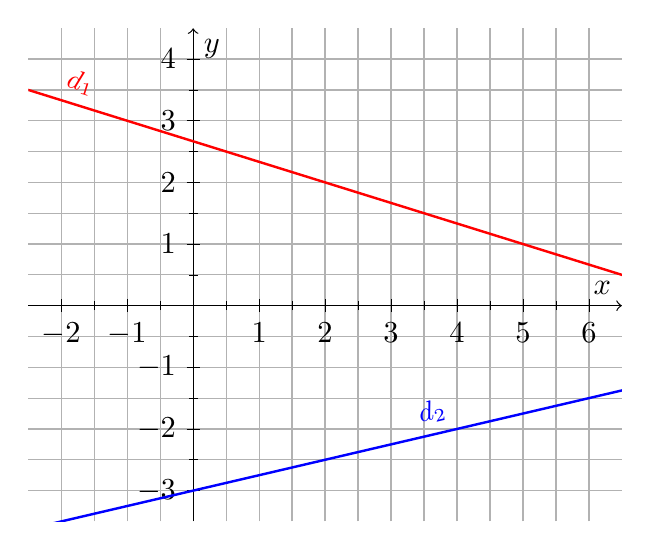
\begin{tikzpicture}[scale=1.1]
    % Define axis
    \begin{axis}[
        axis lines=middle,
        grid=both,
        minor tick num=1,
        xlabel={$x$},
        ylabel={$y$},
        xmin=-2.5, xmax=6.5,
        ymin=-3.5, ymax=4.5,
        xtick={-2,-1,0,1,2,3,4,5,6},
        ytick={-3,-2,-1,0,1,2,3,4},
        axis line style={->},
        tick style={black},
        label style={font=\bfseries},
        grid style={black!30},
    ]
        % Line d1
        \addplot[domain=-4:7, thick, red] { - 1/3*x+8/3} node[pos=0.2, above, sloped] {\small $d_1$};
        \addplot[domain=-4:7, thick, blue] { 1/4*x-3} node[pos=0.7, above, sloped] {\small $d_2$};
    \end{axis}
\end{tikzpicture}
\end{center}}
	\end{minipage}
	\onslide<2->{
	\begin{minipage}[t]{0.4\textwidth}{
	\vspace{0pt}
	Réponses :
	\begin{itemize}
		\item $d_1 : y = -\dfrac{1}{3}x + \dfrac{8}{3}$
		\item $d_2 : y = \dfrac{1}{4}x - 3$
		\item $d_1 \cap d_2=\left(\dfrac{68}{7}; -\dfrac{4}{7}\right)$
	\end{itemize}
	}
\end{minipage}}
\end{frame}
\end{document}
